\section{Technology Assessment}
\label{sec:technology}



Introduce in (sufficient) depth the key concepts and architecture of the chosen software technology. As part if this, you may consider using a running example to introduce the technology.

This part and other parts of the report probably needs to refer to
figures. Figure~\ref{fig:framework} from \cite{brown:96} just
illustrates how figure can be included in the report.

\begin{figure}[thb]
	\centering
	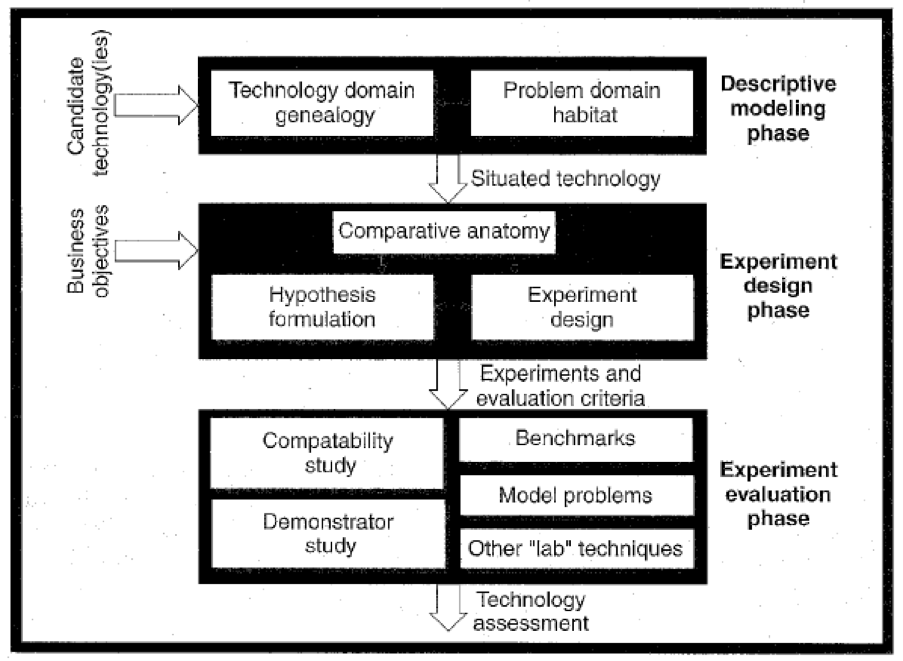
\includegraphics[scale=0.5]{figs/framework.png}
	\caption{Software technology evaluation framework.}
	\label{fig:framework}
\end{figure}

\subsection{Descriptive Modeling}

write where the technology comes from, its history, its context and what problem it solves.
Consider drawing a graph like in \cite{brown:96}.


Kotlin, developed by JetBrains (the Czech software company behind IntelliJ IDEA), is named after Kotlin Island in the Gulf of Finland, near St. Petersburg. JetBrains introduced Kotlin in 2011 as a modern language addressing limitations encountered with Java. The first stable release (Kotlin 1.0) arrived in 2016 and gained quickly gaining traction among Android developers. In 2017, Google endorsed Kotlin as an official language for Android development, a significant boost in adoption. In 2020, JetBrains and Google launched the Kotlin Foundation, solidifying its role in JVM and Android development. Kotlin’s ongoing development focuses on multi-platform capabilities, broadening its use beyond JVM and Android to include web, iOS, and server applications. Kotlin is a statically typed language that compiles to Java bytecode, running on the Java Virtual Machine (JVM), which allows compatibility with Java libraries and frameworks. Designed for safety, conciseness, and interoperability with Java, Kotlin is particularly valuable in three contexts:

\begin{itemize}
    \item \textbf{Android Development}: Kotlin’s concise syntax and enhanced safety features make it a preferred choice in Android development.
    \item \textbf{Server-Side Development}: Kotlin’s seamless integration with JVM-based frameworks like Spring Boot facilitates its use in server applications.
    \item \textbf{Multi-Platform Development}: Kotlin Multiplatform and Kotlin/Native enable shared codebases across platforms, including mobile, web, and desktop applications.
\end{itemize}

\begin{tikzpicture}[node distance=2cm]

\hspace*{-1.5cm}  % Shifts everything 1.5 cm to the left

% Define block styles
\tikzstyle{block} = [rectangle, rounded corners, minimum width=3cm, minimum height=1cm, text centered, draw=black, fill=blue!20]
\tikzstyle{problem} = [rectangle, rounded corners, minimum width=3cm, minimum height=1cm, text centered, draw=black, fill=red!20]
\tikzstyle{context} = [ellipse, minimum width=4cm, minimum height=1cm, text centered, draw=black, fill=yellow!20]
\tikzstyle{arrow} = [thick,->,>=stealth]
\tikzstyle{usecase} = [rectangle, rounded corners, minimum width=3.5cm, minimum height=1cm, text centered, draw=black, fill=green!20]

% Nodes
\node (problem1) [problem,] {Problem 1: Verbose Code};
\node (problem2) [problem, below of=problem1] {Problem 2: Null Safety};
\node (problem3) [problem, below of=problem2] {Problem 3: Complex Asynchronous Code};
\node (context) [context, right of=problem2, xshift=4cm] {Context: Java Development};
\node (kotlin) [block, below of=context, yshift=-1cm] {Kotlin};

% Spread out the blue boxes
\node (feature1) [block, below of=kotlin, xshift=-4cm] {Concise Syntax};
\node (feature2) [block, below of=kotlin] {Null Safety};
\node (feature3) [block, below of=kotlin, xshift=4cm] {Coroutines};

% Spread out the benefits
\node (benefit1) [block, below of=feature1] {Reduced Boilerplate};
\node (benefit2) [block, below of=feature2] {Enhanced Safety};
\node (benefit3) [block, below of=feature3] {Improved Concurrency};

% Use cases (stacked vertically)
\node (usecase1) [usecase, above of=context, xshift=6cm] {Android Development};
\node (usecase2) [usecase, below of=usecase1] {Server-Side Development};
\node (usecase3) [usecase, below of=usecase2] {Multi-Platform Development};

% Arrows
\draw [arrow] (problem1) -- (kotlin);
\draw [arrow] (problem2) -- (kotlin);
\draw [arrow] (problem3) -- (kotlin);
\draw [arrow] (context) -- (kotlin);
\draw [arrow] (kotlin) -- (feature1);
\draw [arrow] (feature1) -- (benefit1);
\draw [arrow] (kotlin) -- (feature2);
\draw [arrow] (feature2) -- (benefit2);
\draw [arrow] (kotlin) -- (feature3);
\draw [arrow] (feature3) -- (benefit3);

% Arrows from use cases to context (yellow oval)
\draw [arrow] (usecase1) -- (context);
\draw [arrow] (usecase2) -- (context);
\draw [arrow] (usecase3) -- (context);

\end{tikzpicture}

\vspace{1cm}

Kotlin is addressing some of Java's limitations. Kotlin is a good programming language in many ways:
\\
\textbf{Conciseness and Readability}: Kotlin’s streamlined syntax reduces repetitive code, improving readability and maintainability. This conciseness also minimizes potential sources of error and makes the codebase easier to work with.

\textbf{Null Safety}: Kotlin’s type system helps prevent NullPointerExceptions by distinguishing between nullable and non-nullable types. This feature significantly reduces bugs related to null handling, a frequent issue in Java.

\textbf{Interoperability with Java}: Kotlin’s full compatibility with Java allows teams to gradually integrate Kotlin into existing Java applications. This flexibility is advantageous for modernization efforts without requiring a complete code rewrite.

\textbf{Asynchronous Programming with Coroutines}: Kotlin’s coroutines offer a simplified approach to asynchronous programming, enabling more efficient, non-blocking code execution ideal for network requests or tasks involving resource waits.

\textbf{Multi-Platform Support}: Kotlin’s multiplatform capabilities allow for shared business logic across platforms, reducing code duplication and streamlining development for applications targeting Android, iOS, web, and server environments.

\textbf{Functional Programming Features}: Kotlin includes extension functions, higher-order functions, and lambdas, allowing more expressive, modular code. These features support functional programming, further enhancing code flexibility and promoting cleaner architecture.

\textbf{Data Classes}: Kotlin’s data classes simplify the creation of classes primarily used for holding data by automatically generating common methods like \texttt{equals()}, \texttt{hashCode()}, and \texttt{toString()}, streamlining data handling.


\subsection{Experiment Design}

Write you hypotheses about what benefits the technology bring and how you can support or reject them via experiments.

\maketitle

\section*{Improved Development Speed and Code Conciseness}

\textbf{Hypothesis:} Using Kotlin will reduce development time due to its concise syntax. This is expected to simplify tasks such as user, poll, and vote management.

\textbf{Experiment:} Compare the implementation time for key functionalities (e.g., user creation, poll management, and vote handling) between Kotlin and Java. Measure the lines of code required to implement the same logic in both languages and track developer productivity through task completion rates.

\section*{Enhanced Safety with Null Safety}

\textbf{Hypothesis:} Kotlin’s null safety features will reduce runtime exceptions related to null pointer errors, especially in scenarios where entities (like User, Poll, or Vote) might not exist, which would otherwise cause crashes in Java.

\textbf{Experiment:} Introduce null values in critical parts of the business logic (e.g., missing users or votes) and measure the number of runtime exceptions in both Kotlin and Java. Monitor the resilience of the application in handling missing data.

\section*{Simplified Asynchronous Voting Process}

\textbf{Hypothesis:} Kotlin coroutines will streamline asynchronous handling of voting logic, improving response time and scalability during high voting activity.

\textbf{Experiment:} Implement the voting logic using Kotlin coroutines, then simulate high volumes of voting requests. Compare the application’s response times and memory usage with a similar Java implementation using standard concurrency methods.

\section*{Cross-Platform Code Sharing Potential}

\textbf{Hypothesis:} Kotlin Multiplatform would enable code sharing for the voting logic between a potential mobile client and backend, reducing duplicated logic and ensuring consistency across platforms.

\textbf{Experiment:} Set up a prototype of a shared code module containing core voting functions for both the backend and an Android client. Measure code duplication and maintenance requirements, assessing potential consistency improvements.


\subsection{Experiment Evaluation}

Write about the results of your experiments, either via personal experience reports, quantitative benchmarks, a demostrator case study or a combination of multiple approaches.


For some reports you may have to include a table with experimental
results are other kinds of tables that for instance compares
technologies. Table~\ref{tab:results} gives an example of how to create a table.

\begin{table}[bth]
	\centering
	\begin{tabular}{llrrrrrr}
		Config & Property & States & Edges & Peak & E-Time & C-Time & T-Time
		\\ \hline \hline
		22-2 & A   &    7,944  &   22,419  &  6.6  \%  &  7 ms & 42.9\% &  485.7\% \\
		22-2 & A   &    7,944  &   22,419  &  6.6  \%  &  7 ms & 42.9\% &  471.4\% \\
		30-2 & B   &   14,672  &   41,611  &  4.9  \%  & 14 ms & 42.9\% &  464.3\% \\
		30-2 & C   &   14,672  &   41,611  &  4.9  \%  & 15 ms & 40.0\% &  420.0\% \\ \hline
		10-3 & D   &   24,052  &   98,671  & 19.8  \%  & 35 ms & 31.4\% &  285.7\% \\
		10-3 & E   &   24,052  &   98,671  & 19.8  \%  & 35 ms & 34.3\% &  308.6\% \\
		\hline \hline
	\end{tabular}
	\caption{Selected experimental results on the communication protocol example.}
	\label{tab:results}
\end{table}
